\begin{frame}{ML-Blink UI Implementation}
    \begin{itemize}
        \item Allows to match images of distinct datasets of the same location in the night sky
    \end{itemize}
\end{frame}

\begin{frame}{ML-Blink UI Implementation}
    \begin{itemize}
        \item Allows to match images of distinct datasets of the same location in the night sky
        \item Goal is to provide intuitive feedback about the quality of the current matching 
    \end{itemize}
\end{frame}

\begin{frame}{ML-Blink UI Implementation}
    \begin{itemize}
        \item Allows to match images of distinct datasets of the same location in the night sky
        \item Goal is to provide intuitive feedback about the quality of the current matching 
        \item The matching algorithm
            \begin{itemize}
                \item Computing the region of interest (ROI)
                \item Smoothing
                \item Binarization
                \item Object detection
                \item Object size normalization
                \item Computing accuracy
            \end{itemize}
    \end{itemize}
\end{frame}

\begin{frame}{ML-Blink UI Implementation}
    \begin{figure}[H]
        \centering
        \begin{subfigure}{.5\textwidth}
          \centering
          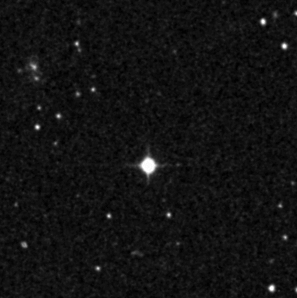
\includegraphics[
                width=0.9\textwidth,
                height=\textheight,
                keepaspectratio
            ]{report/images/image-matching/usno-0-blue1.png}
          \caption{\usno}
        \end{subfigure}%
        \begin{subfigure}{.5\textwidth}
          \centering
          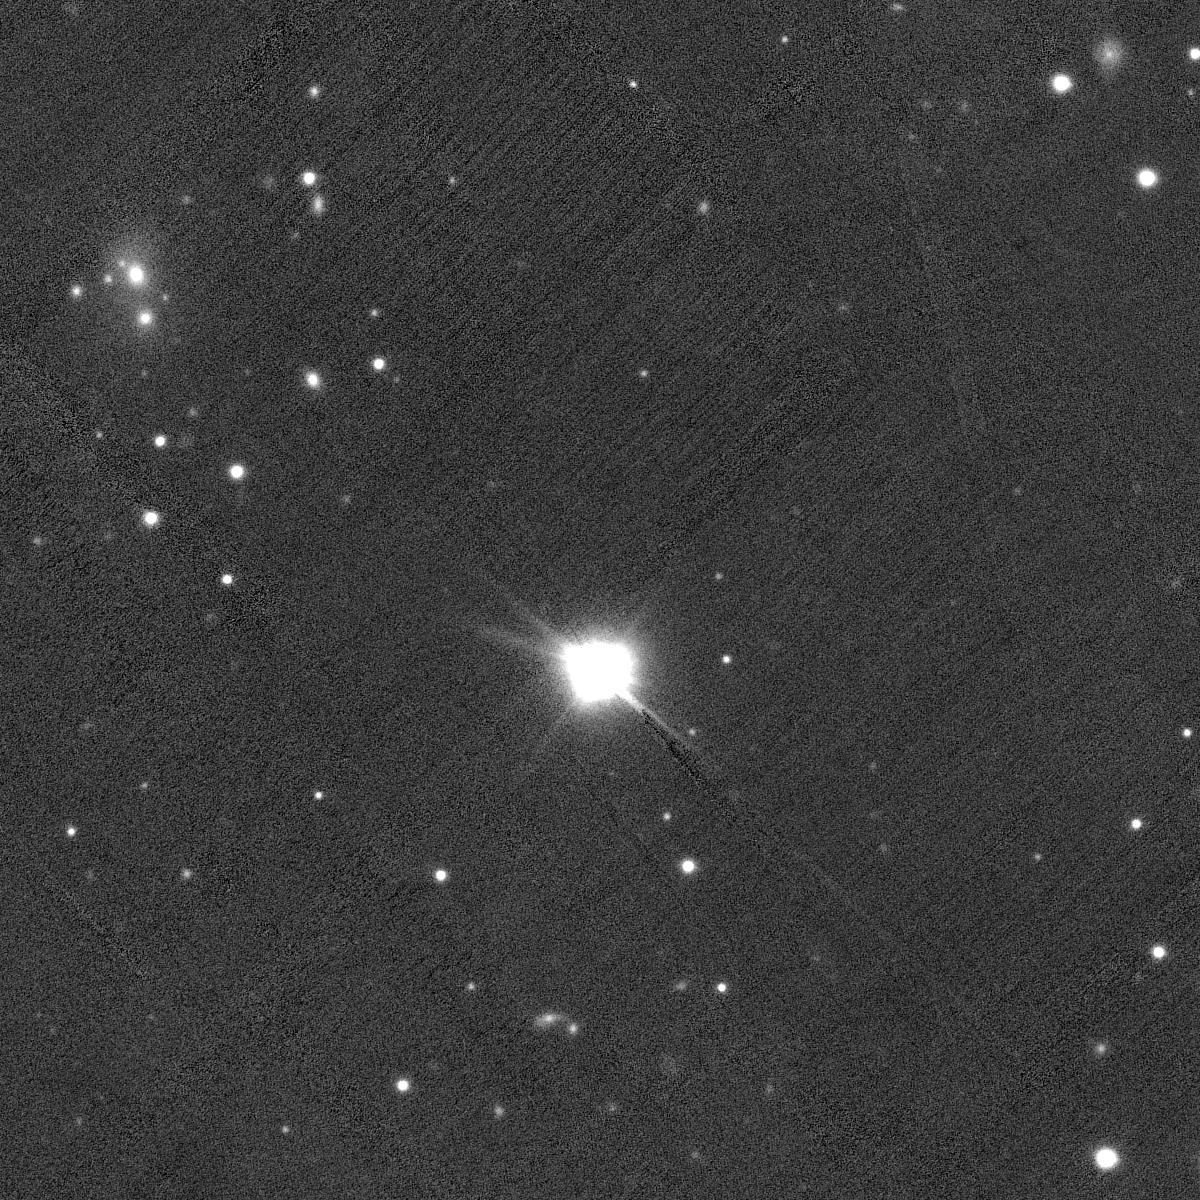
\includegraphics[
                width=0.9\textwidth,
                height=\textheight,
                keepaspectratio
          ]{report/images/image-matching/panstarr-0-g.png}
          \caption{\panstarrs}
        \end{subfigure}
        \caption{Pictures taken from the same location in the night sky from \usno and \panstarrs respectively.}
    \end{figure}
\end{frame}

\begin{frame}{ROI}
    \begin{figure}[H]
        \centering
        \begin{subfigure}{.5\textwidth}
          \centering
          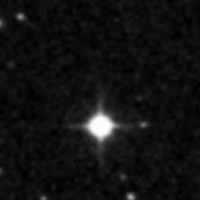
\includegraphics[
                width=0.75\textwidth,
                height=\textheight,
                keepaspectratio
            ]{report/images/image-matching/usno-0-blue1-roi.png}
          \caption{\usno ROI}
        \end{subfigure}%
        \begin{subfigure}{.5\textwidth}
          \centering
          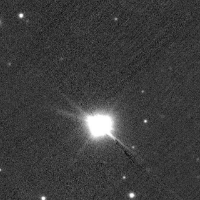
\includegraphics[
                width=0.75\textwidth,
                height=\textheight,
                keepaspectratio
          ]{report/images/image-matching/panstarr-0-g-roi.png}
          \caption{\panstarrs ROI}
        \end{subfigure}
        \caption{The ROI is computed as if the \panstarrs image was placed exactly on top of the \usno image in the UI.}
    \end{figure}
\end{frame}

\begin{frame}{Smoothing}
    \begin{itemize}
        \item Pixel value intensities are smoothed using a mean filter
    \end{itemize}
\end{frame}

\begin{frame}{Smoothing}
    \begin{itemize}
        \item Pixel value intensities are smoothed using a mean filter
        \item Facilitates object detection later on
    \end{itemize}
\end{frame}

\begin{frame}{Smoothing}
    \begin{itemize}
        \item Pixel value intensities are smoothed using a mean filter
        \item Facilitates object detection later on
        \item $3 \times 3$ kernel that scans the entire ROI
    \end{itemize}
\end{frame}

\begin{frame}{Smoothing}
    \begin{itemize}
        \item Pixel value intensities are smoothed using a mean filter
        \item Facilitates object detection later on
        \item $3 \times 3$ kernel that scans the entire ROI
        \item Mean pixel value intensity of the entire ROI is used for out--of--boundary pixels
    \end{itemize}
\end{frame}

\begin{frame}{Binarization}
    \begin{figure}[H]
        \centering
        \begin{subfigure}{.5\textwidth}
          \centering
          
\includegraphics[
                width=0.75\textwidth,
                height=\textheight,
                keepaspectratio
            ]{report/images/image-matching/usno-0-blue1-bw.png}
          \caption{Binarized \usno}
        \end{subfigure}%
        \begin{subfigure}{.5\textwidth}
          \centering
          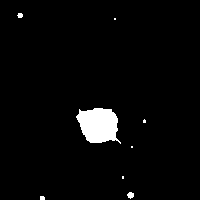
\includegraphics[
                width=0.75\textwidth,
                height=\textheight,
                keepaspectratio
          ]{report/images/image-matching/panstarr-0-g-bw.png}
          \caption{Binarized \panstarrs}
        \end{subfigure}
        \caption{Binarization result using a threshold value of 80 for \usno and 110 for \panstarrs.}
    \end{figure}
\end{frame}

\begin{frame}{Object Detection}
    \begin{figure}[H]
        \centering
        \begin{subfigure}{.5\textwidth}
          \centering
          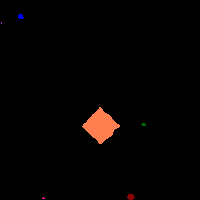
\includegraphics[
                width=0.75\textwidth,
                height=\textheight,
                keepaspectratio
            ]{report/images/image-matching/usno-0-blue1-objects.png}
          \caption{Objects in \usno}
        \end{subfigure}%
        \begin{subfigure}{.5\textwidth}
          \centering
          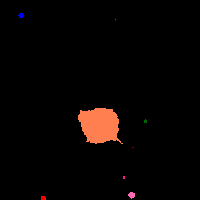
\includegraphics[
                width=0.75\textwidth,
                height=\textheight,
                keepaspectratio
          ]{report/images/image-matching/panstarr-0-g-objects.png}
          \caption{Objects in \panstarrs}
        \end{subfigure}
        \caption{Object detection result for both \usno  and \panstarrs.}
    \end{figure}
\end{frame}

\begin{frame}{Object Size Normalization}
    \begin{figure}[H]
        \centering
        \begin{subfigure}{.5\textwidth}
          \centering
          
\includegraphics[
                width=0.75\textwidth,
                height=\textheight,
                keepaspectratio
            ]{report/images/image-matching/usno-0-blue1-equal-sized-objects.png}
          \caption{Equal sized objects in \usno}
        \end{subfigure}%
        \begin{subfigure}{.5\textwidth}
          \centering
          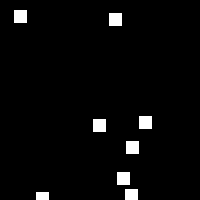
\includegraphics[
                width=0.75\textwidth,
                height=\textheight,
                keepaspectratio
          ]{report/images/image-matching/panstarr-0-g-equal-sized-objects.png}
          \caption{Equal sized objects in \panstarrs}
        \end{subfigure}
        \caption{Original objects replaced by equal sized objects in \usno  and \panstarrs. Squared objects of size $9$ are used for \usno images and $13$ for \panstarrs images.}
    \end{figure}
\end{frame}

\begin{frame}{Accuracy}
    \begin{itemize}
        \item Number of remaining bright pixel value intensities when the \usno image is subtracted from the \panstarrs image
    \end{itemize}
\end{frame}

\begin{frame}{Accuracy}
    \begin{itemize}
        \item Number of remaining bright pixel value intensities when the \usno image is subtracted from the \panstarrs image
        \item Let \usno image be $\text{xs}$, \panstarrs image $\text{ys}$, and $\text{zs} = \text{xs} - \text{ys}$
    \end{itemize}
\end{frame}

\begin{frame}{Accuracy}
    \begin{itemize}
        \item Number of remaining bright pixel value intensities when the \usno image is subtracted from the \panstarrs image
        \item Let \usno image be $\text{xs}$, \panstarrs image $\text{ys}$, and $\text{zs} = \text{xs} - \text{ys}$
        \item 
            \begin{equation}
                \text{accuracy} = 100 - \frac{|\text{zs} \in \{255\} | \times 100}{|\text{xs} \in \{255\} |}
            \end{equation}
    \end{itemize}
\end{frame}